\documentclass{standalone}
\usepackage{tikz}
\begin{document}
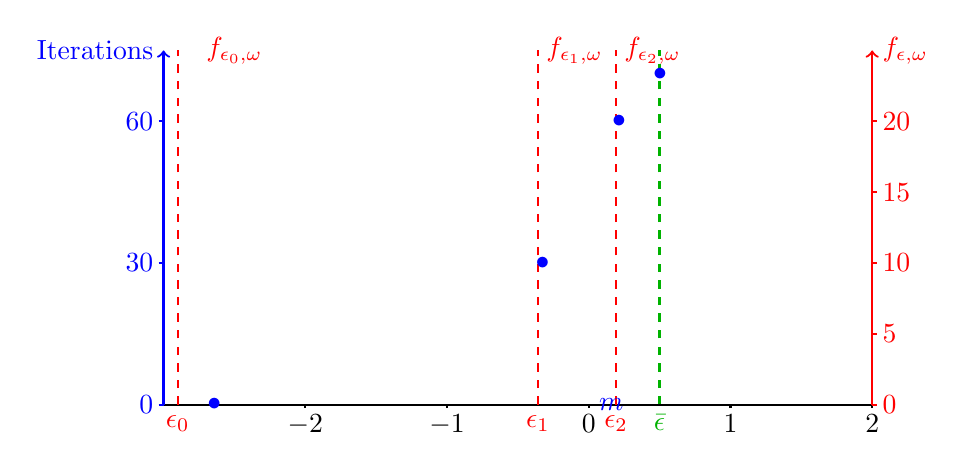
\begin{tikzpicture}[yscale = 0.06, xscale = 1.8, thick]
  %\node at (-1.4, 40) {\Large $\displaystyle J^{\min} = \min_{e,j} \frac{J_{ej}}{J_e^0}$};
  \draw[dashed, green!70!black](0.5, 0) node[below]{$\bar{\epsilon}$}-- (0.5, 75);
  \begin{scope}[black]
    \draw(-3,0) -- (2,0) node[right] {};
    \foreach \x in {-2, -1, 0, 1, 2}
      \draw[shift={(\x, 0)}] node[below] {$\x$}(0pt, -20pt) -- (0pt,0pt) ;
  \end{scope}
  \begin{scope}[red, yscale = 3]
    \draw[dashed](-2.9, 0) node[below]{$\epsilon_0$}-- (-2.9, 25) ;
    \draw[dashed](-0.358, 0) node[below]{$\epsilon_1$}-- (-0.358, 25);
    \draw[dashed](0.193, 0) node[below]{$\epsilon_2$}-- (0.193, 25);
    \begin{scope}
      \clip(-3.5, 0) rectangle(2.4, 25);
      \draw[domain = -3:2, samples=500] plot[id=opti1] function{(log((x + 2.9)/ 3.9))**2 + (x - 1)**2}; 
      \draw[domain = -3:2, samples=500] plot[id=opti2] function{(log((x + 0.358)/ 1.358))**2 + (x - 1)**2}; 
      \draw[domain = -3:2, samples=500] plot[id=opti3] function{(log((x - 0.193)/ 0.807))**2 + (x - 1)**2}; 
    \end{scope}
    \node at (-2.50, 25) {$f_{\epsilon_0,\omega}$};
    \node at (-0.10, 25) {$f_{\epsilon_1,\omega}$};
    \node at (0.45, 25) {$f_{\epsilon_2,\omega}$};
    \foreach \y in {0, 5, 10, 15, 20}
      \draw[shift={(2, \y)}] node[right] {$\y$}(0pt, 0pt) -- (1pt,0pt) ;
    \draw[->] (2,0) -- (2,25) node[right] {$f_{\epsilon,\omega}$};
  \end{scope}
  \begin{scope}[blue]
    \draw plot file {opti2.dat} node[right]{$m$};
    \node at (-2.641, 0) {$\bullet$};
    \node at (-0.3257, 30) {$\bullet$};
    \node at (0.214, 60) {$\bullet$};
    \node at (0.5025, 70) {$\bullet$};
    \draw[->] (-3,0) -- (-3,75) node[left] {Iterations};
    \foreach \y in {0, 30, 60}
      \draw[shift={(-3, \y)}] node[left] {$\y$}(-1pt, 0pt) -- (0pt,0pt) ;
  \end{scope}
\end{tikzpicture}
\end{document}
